\section{Introduction}
DNA-encoded chemical libraries (DELs) enable the synthesis of billion-member compound collections and the screening of vast chemical spaces that would be difficult to access with conventional high-throughput screening\cite{brenner_encodedcombinatorialchemistry_1992,franzini_dnaencodedchemicallibraries_2014,favalli_dnaencodedchemicallibraries_2018,neri_dnaencodedchemicallibraries_2018,fitzgerald_dnaencodedchemistrydrug_2021,keller_impactdnaencodedchemical_2022,satz_dnaencodedchemicallibraries_2022,peterson_smallmoleculediscoverydnaencoded_2023,wichert_challengesprospectsdnaencoded_2024}. In analogy to biological display technologies, each library member is linked to an encoding DNA sequence, which connects phenotype (the small molecule) to genotype (the DNA tag). This design enables the parallel screening of very large libraries against biological targets and supports efficient hit discovery\cite{neri_dnaencodedchemicallibraries_2018,huang_strategiesdevelopingdnaencoded_2022}.

Affinity-based DEL selections can be automated and have been described previously in Nature Protocols\cite{decurtins_automatedscreeningsmall_2016}. After selection, the DNA tags of retained compounds are PCR-amplified and analyzed by high-throughput sequencing to determine the abundance of individual library members\cite{decurtins_automatedscreeningsmall_2016,satz_dnaencodedchemicallibraries_2022}. DELs are now used widely in both industry and academia\cite{satz_dnaencodedchemicallibraries_2022,peterson_smallmoleculediscoverydnaencoded_2023,wichert_challengesprospectsdnaencoded_2024,goodnow_dnaencodedchemistryenabling_2017}.

DEL architectures include single-display and dual-display formats, depending on whether the pharmacophore is presented on one DNA-linked fragment or on two pairing oligonucleotide strands\cite{lessing_advancingsmallmoleculedrug_2023}. Standard libraries are often encoded on double-stranded DNA headpieces, but single-stranded and Y-shaped encoding schemes are also used\cite{plais_universalencodingnext_2022}. Regardless of the encoding format, selection and PCR amplification ultimately produce double-stranded amplicons for DNA sequencing and downstream analysis\cite{decurtins_automatedscreeningsmall_2016}.

DEL datasets require the integration of sequence processing, cheminformatics, and statistical analysis, while offering unique opportunities for machine-learning-based modeling and discovery\cite{franzini_chemicalspacednaencoded_2016,mccloskey_machinelearningdnaencoded_2020,reiher_trendshittoleadoptimization_2021,shi_recentadvancesdnaencoded_2022,hou_machinelearningbaseddataanalysis_2023,shmilovich_deldockmoleculardockingenabled_2023,torng_deeplearningapproach_2023,edfeldt_datascienceroadmap_2024,edwards_proteinliganddata_2025,montoya_widespreadfalsenegatives_2025,sigel_dnaencodedlibrarymachine_2025,wang_rationaldesignstrategies_2025,gampe_analysesrecenthitfinding_2026}.
At the same time, DEL analysis poses challenges that are not addressed by standard genomics workflows, including demultiplexing complex barcode combinations, reconstructing chemical structures from encoded building blocks, comparing enrichment across conditions, and connecting selection outputs to downstream structure-based analysis.

Individual components of a DEL analysis workflow can be assembled from tools originally developed for cheminformatics and bioinformatics workflows, but these tools do not readily support the diversity of DEL architectures and experimental designs encountered in practice. In addition, they typically lack DEL-specific intermediate outputs and quality-control measures that facilitate troubleshooting, validation, and interpretation of results.


\subsection{Development of the protocol}
We developed DELT-Hit to support routine analysis of DEL campaigns across a wide range of library sizes and architectures.
The workflow combines and extends established tools and methods with DEL-specific sequence handling, chemical enumeration,
and quality control. Configuration files and standardized outputs support reproducibility, while the modular design allows
users to adapt the workflow to different experimental settings.


\begin{figure}[htbp]
\centering
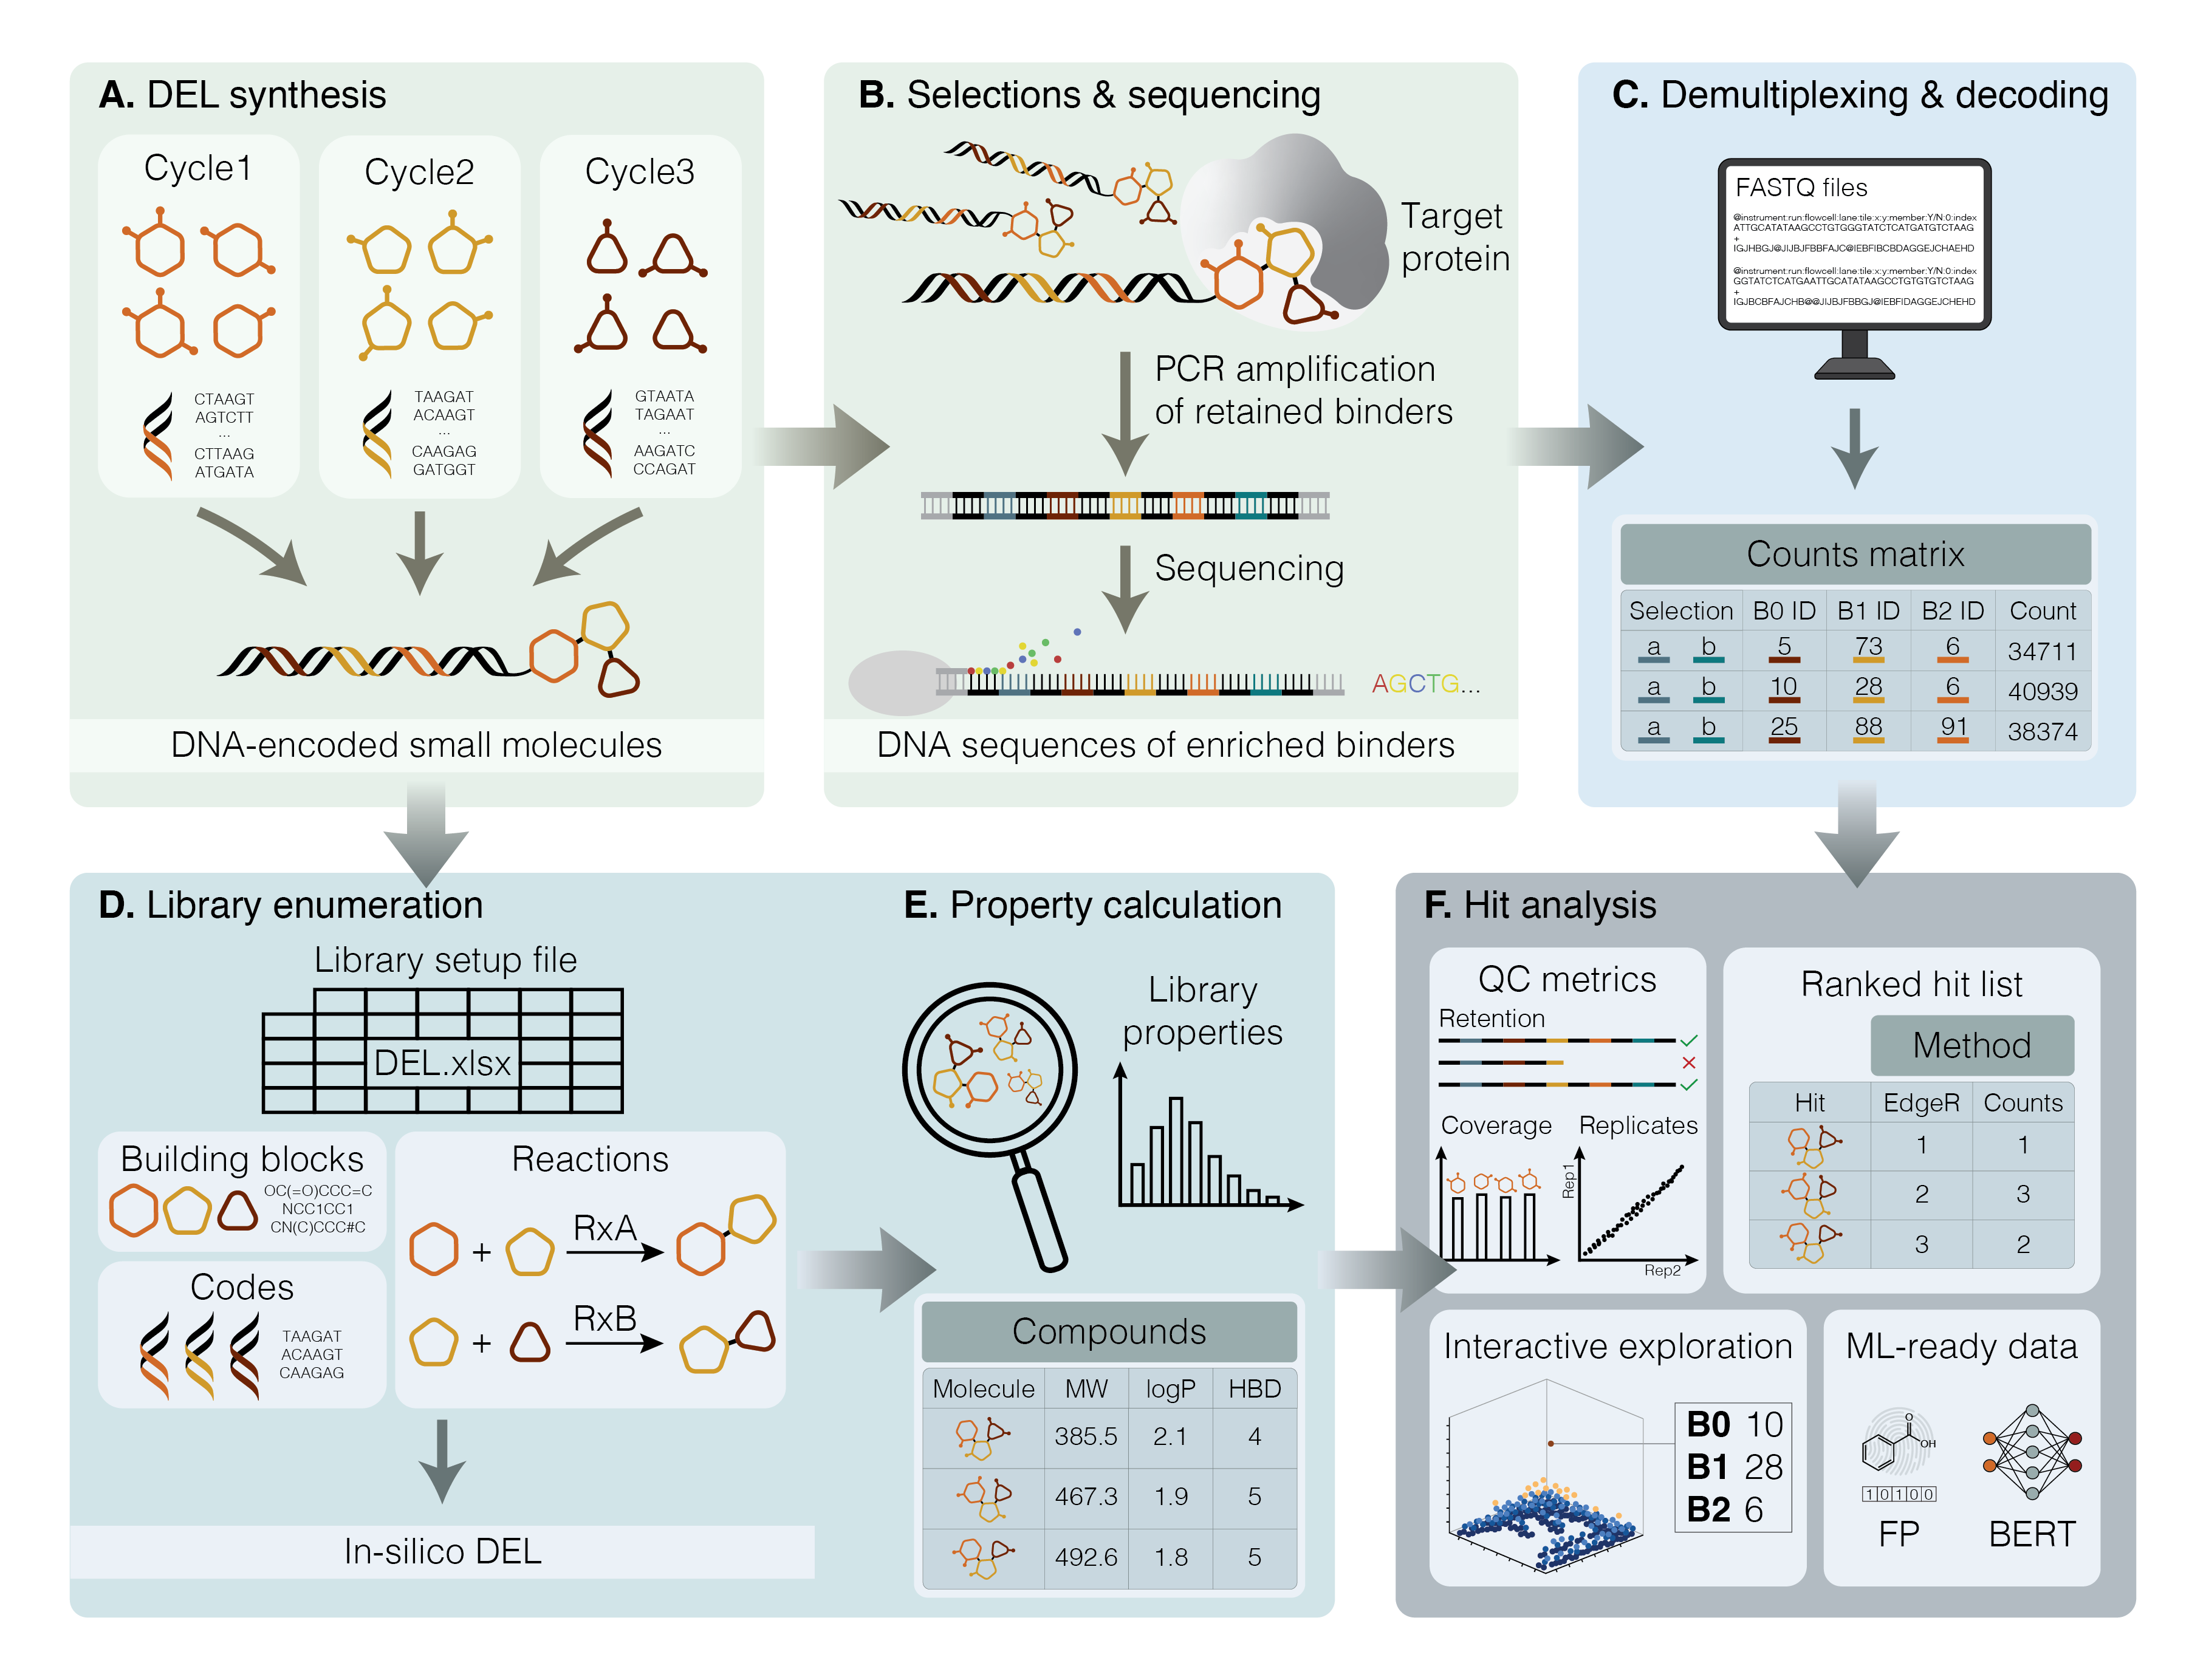
\includegraphics[width=\textwidth]{figures/workflow-overview.png}
\caption{DELT-Hit is organized into several modules (C - F) that complement the wet-lab DEL workflow (A - B). DEL synthesis (A) proceeds through iterative cycles of building block addition and encoding. Libraries are then screened in affinity-based selection experiments (B), after which retained DNA tags are PCR-amplified and sequenced. DELT-Hit uses Cutadapt\cite{martin_cutadaptremovesadapter_2011} to demultiplex sequencing reads (C) with user-defined error tolerances and produces count matrices for combinations of selection and building block codes. In parallel, library compounds can be enumerated in silico (D) from building block structures and reaction SMIRKS definitions, and molecular properties can be calculated (E). These in silico enumeration and property-calculation features can be applied before DEL synthesis to support library design and building-block selection. DELT-Hit subsequently integrates count data and chemical information for hit analysis (F), quality control, enrichment ranking, and interactive data exploration. In addition, the workflow exports molecular representations, including Morgan fingerprints and BERT embeddings, for downstream machine-learning applications.}
\label{fig:figure1}
\end{figure}
Figure~\ref{fig:figure1} summarizes the overall DELT-Hit workflow. The workflow integrates sequence demultiplexing via Cutadapt\cite{martin_cutadaptremovesadapter_2011}, chemical structure representation in SMILES\cite{weininger_smileschemicallanguage_1988,weininger_smiles2algorithm_1989,weininger_smiles3depict_1990}, reaction definitions in SMIRKS\cite{ref33,ref34} implemented in RDKit\cite{landrum_rdkitrdkit2025_09_4_2025}, different enrichment-analysis methods including edgeR\cite{robinson_edgerbioconductorpackage_2010}, molecular property calculation, library-member enumeration, and interactive visualization. Users can run the full workflow or individual modules, and each stage produces executable scripts and standardized outputs that can be adapted to more specialized analyses.


\subsection{Overview of the procedure}
The DELT-Hit protocol is organized into six analysis phases spanning 20 steps. Some downstream phases are optional or can be run independently:

(i) Project setup and library specification (Steps 1--9): Configuration file creation from Excel templates, library architecture definition, reaction specification, and experimental metadata setup.

(ii) Sequence demultiplexing and quality assessment (Steps 10--12): High-throughput sequencing data processing, barcode identification with error correction, and quality-control metric generation.

(iii) Data visualization and interpretation (Step 13): Interactive dashboard exploration of raw count data to identify selections of interest.

(iv) Selection enumeration and enrichment analysis (Steps 14--15): Automated SMILES generation and molecular property calculation for the top enriched compounds of a chosen selection.

(v) Statistical analysis and hit detection (Steps 16--17): Enrichment analysis using established RNA-seq methods, hit ranking with multiple statistical approaches, and result validation.

(vi) Full library enumeration and machine-learning representations (Steps 18--20): Optional full-library enumeration and generation of molecular fingerprints and embeddings for downstream machine-learning workflows.


\subsection{Applications of the method}
DELT-Hit accommodates library architectures ranging from simple two-cycle libraries to more complex multi-branch schemes. The workflow has been applied across several DEL campaigns:

A single-display DEL with two diversity elements comprising 366,600 glutamic acid derivatives (GB-DEL) was encoded in a single-display DNA format and tested in affinity-based selections, enabling de novo identification of binders against several pharmaceutically relevant proteins. The GB-DEL was also used for affinity maturation in a dual-display format by combining it with low-affinity hits displayed on a pairing strand\cite{bassi_singlestrandeddnaencodedchemical_2020}.

A second single-display DEL with two diversity elements comprising 670,752 derivatives based on a 2-azido-3-iodophenylpropionic acid scaffold (NF-DEL) was likewise encoded in a single-display DNA format and used to investigate the effect of stereo- and regiochemistry on ligand discovery. Selections against pharmaceutically relevant protein targets yielded selective enzyme inhibitors and binders to tumor-associated antigens that enabled conditional chimeric antigen receptor T-cell activation and tumor targeting\cite{favalli_stereoregiodefineddnaencoded_2021}.

A proof-of-principle single-display, double-stranded DEL containing 1,100 members and three amino acid diversity elements was synthesized on magnetic beads using a solid-phase approach with final release of the library from the support. The workflow supported analysis of both the standard released library and a self-purified version in which incomplete synthetic structures were removed before final release. Selections against carbonic anhydrase II and IX showed improved enrichment of the positive control for the self-purified DEL. Because synthesis and encoding yields correlate in this format, DNA sequencing of the unselected library can be used to assess chemical display yields. The solid-support synthesis also permits anhydrous reaction conditions and therefore enables water-free chemistry that is difficult to implement in standard DEL workflows\cite{keller_highlypurednaencoded_2024}.

A dual-display encoded self-assembling chemical (ESAC) library containing 56 million members enabled incremental connection of two displayed peptides. This library was used to study macrocycle flexibility with a two-step cyclization strategy. Selections against three targets revealed target-specific preferences for different conformational states, including a 314 nM thrombin inhibitor from the conformationally restrained macrocyclic subset, a more flexible streptavidin binder from the semi-closed conformation, and binders to human alkaline phosphatase (PLAP) from the open dual-display format\cite{petrov_flexibilitytuningdualdisplaydnaencoded_2025}.

The low- and medium-complexity studies presented here can be analyzed with DELT-Hit in less than 2 hours. Re-analyses of the published datasets from Favalli et al. and Keller et al. are summarized in Supplementary Note~\ref{supp:analysis-of-published-datasets}.

\subsection{Limitations}
While DELT-Hit addresses many challenges in DEL analysis, several limitations should be considered:

\begin{itemize}
  \item Computational complexity: Library size grows combinatorially with the number of diversity elements, primarily affecting library enumeration, property calculation, and molecular representation. In contrast, demultiplexing depends mainly on the number of sequencing reads (sequencing depth) and is therefore largely independent of library size. Although full enumeration of extremely large libraries can become computationally prohibitive, DELT-Hit supports selective enumeration of compounds detected in the individual selection experiments, substantially reducing computational requirements.
  \item Library chemistry: DELT-Hit supports arbitrary synthetic routes, provided that each route yields a single, well-defined final product. Libraries with non-standard reaction schemes, unconventional building block representations, or complex precursor handling may require additional configuration and validation. Accurate reaction SMIRKS definitions are essential for correct enumeration and require cheminformatics expertise.
\end{itemize}

\subsection{Comparison with other methods}

\newcommand{\statusgreen}{\raisebox{0.15ex}{\textcolor{green!50!black}{\LARGE$\bullet$}}}
\newcommand{\statusamber}{\raisebox{0.15ex}{\textcolor{orange!90!black}{\LARGE$\bullet$}}}
\newcommand{\statusopen}{\raisebox{0.15ex}{\textcolor{black!30}{\LARGE$\bullet$}}}
\newcommand{\statusred}{\raisebox{0.15ex}{\textcolor{blue!70!black}{\LARGE$\bullet$}}}
\begin{longtable}{p{8.8cm}>{\centering\arraybackslash}p{2.8cm}>{\centering\arraybackslash}p{1.2cm}}
\caption{Comparison of DELT-Hit and DELi\cite{wellnitz_opensourcednaencodedlibrary_2025} across selected scientific-software criteria. \statusgreen\ supported; \statusamber\ partial support; \statusopen\ not clearly documented; \statusred\ not supported.}
\label{tab:delt-deli-comparison} \\
\toprule
\textbf{Criterion} & \textbf{DELT-Hit} & \textbf{DELi} \\
\midrule
\endfirsthead

\toprule
\textbf{Criterion} & \textbf{DELT-Hit} & \textbf{DELi} \\
\midrule
\endhead

\multicolumn{3}{l}{\textbf{1. Workflow scope and usability}} \\
1.1 Library design support & \statusamber & \statusgreen \\
1.2 Configuration and workflow ergonomics & \statusgreen & \statusgreen \\
1.3 Interoperability and downstream reuse & \statusgreen & \statusamber \\
\midrule
\multicolumn{3}{l}{\textbf{2. Supported DEL architectures}} \\
2.1 Single-display support & \statusgreen & \statusgreen \\
2.2 Dual-display support & \statusgreen & \statusopen \\
\midrule
\multicolumn{3}{l}{\textbf{3. Decoding and sequencing-side QC}} \\
3.1 Error-tolerant demultiplexing & \statusgreen & \statusgreen \\
3.2 UMI-aware counting & \statusamber & \statusgreen \\
3.3 Decoding QC and reporting & \statusgreen & \statusgreen \\
\midrule
\multicolumn{3}{l}{\textbf{4. Chemical reconstruction and enumeration}} \\
4.1 Library enumeration & \statusgreen & \statusgreen \\
4.2 Flexible reaction-scheme support & \statusgreen & \statusred \\
\midrule
\multicolumn{3}{l}{\textbf{5. Statistical analysis and hit interpretation}} \\
5.1 Count-based enrichment & \statusgreen & \statusgreen \\
5.2 Statistical enrichment scoring & \statusgreen & \statusgreen \\
5.3 Synthon-level analysis & \statusred & \statusgreen \\
\midrule
\multicolumn{3}{l}{\textbf{6. Computational performance}} \\
6.1 Memory and scaling behavior & \statusgreen & \statusamber \\
\bottomrule
\end{longtable}

Pharmaceutical companies that run DEL campaigns typically use internal or licensed software platforms that integrate sequencing, barcode decoding, hit identification, and downstream prioritization within proprietary ecosystems. These systems can support scalability and automation, but they are closed-source and therefore limit methodological transparency, user-driven customization, and community-led improvement.

Contract research organizations (CROs) also provide DEL screening as a service against user-supplied targets. These services usually return processed results without exposing the underlying computational workflow or intermediate data products. As a result, users have limited opportunity to adapt the analysis, inspect intermediate outputs, or integrate DEL informatics into their own pipelines.

To our knowledge, DELi\cite{wellnitz_opensourcednaencodedlibrary_2025} is the only other open-source software package that combines barcode decoding, enrichment analysis, and library enumeration. DELi and DELT-Hit share several design principles, including modular architecture, transparent configuration, and integration with established bioinformatics and cheminformatics tools such as Cutadapt and RDKit (Table~\ref{tab:delt-deli-comparison}). DELT-Hit differs in several areas:

\begin{itemize}
  \item support for complex reaction paths,
  \item integration of RNA-seq-derived statistical models for hit calling that account for replicate structure and dispersion,
  \item support for widely used library designs, including single-display and dual-display formats.
\end{itemize}

DELT-Hit also exposes intermediate data products and executable scripts, allowing users to inspect, adapt, and extend each analysis step for reproducible benchmarking and integration. Furthermore, DELT-Hit exhibits substantially more favorable runtime and memory complexity than DELi, enabling the analysis of industry-scale libraries with billions of sequencing reads. A more detailed comparison of DELT-Hit and DELi is provided in Supplementary Note~\ref{supp:comparison-delt-deli}.
